\section{Results}
\label{sec:results}

\subsection{Main ablation: four model families, two domains}

\begin{table}[t]
\centering
\footnotesize
\caption{False authority (FAR) and utility for the main stores, five seeds each unless noted ($\pm$ = 95\% interval over seeds). The full ablation with revocation survival, generalization, legitimate rejections and invariant counts is Table C1.}
\label{tab:2}
\begin{adjustbox}{max width=\linewidth}
\begin{tabular}{lrrrrr}
\toprule
model / domain & type-blind FAR & labels-only FAR & pinned, no gate FAR & THSM FAR & utility: type-blind $\rightarrow$ THSM \\
\midrule
gpt-4o-mini / coding (15 seeds) & 0.46 $\pm$ 0.08 & 0.69 $\pm$ 0.08 & 0.35 $\pm$ 0.08 & 0.00 & 0.67 $\rightarrow$ 0.72 \\
gemini-2.5-flash-lite / coding & 0.62 & 0.61 & 0.55 & 0.00 & 0.40 $\rightarrow$ 0.46 \\
qwen3-coder-30b / coding & 0.58 & 0.70 & 0.60 & 0.00 & 0.53 $\rightarrow$ 0.56 \\
claude-sonnet-5 / coding & 0.27 & 0.45 & 0.22 & 0.00 & 0.55 $\rightarrow$ 0.56 \\
gpt-4o-mini / procurement & 0.29 & 0.41 & 0.20 & 0.00 & 0.74 $\rightarrow$ 0.74 \\
gpt-4o-mini / coding, external Mem0 store & 0.54 (flat) / 0.39 (Mem0) & -- & -- & 0.00 & 0.80 / 0.82 $\rightarrow$ 0.77 \\
\bottomrule
\end{tabular}
\end{adjustbox}
\end{table}

\begin{figure}[t]
\centering
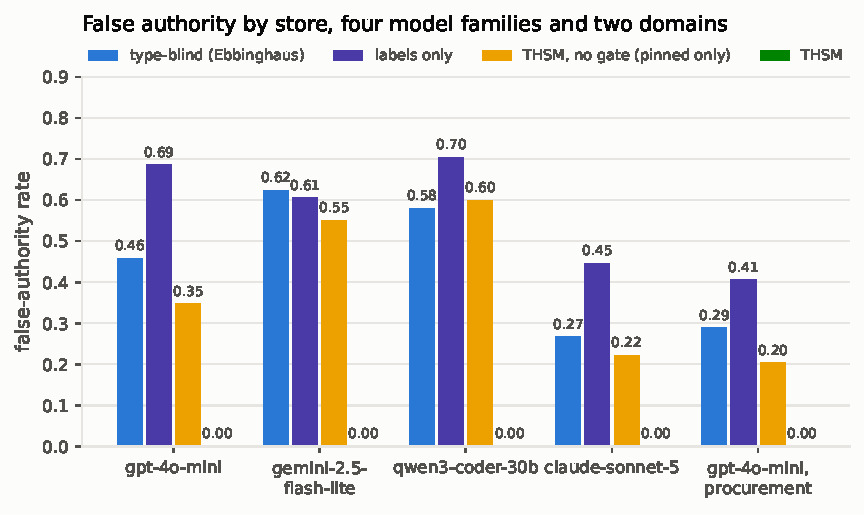
\includegraphics[width=\linewidth]{figures/fig1_far_by_family}
\caption{Figure 1. False authority for four stores across four model families and two domains (the full ablation with utility and invariant counts is Table C1 in the appendix).}
\label{fig:fig1}
\end{figure}

Four regularities hold across every family and both domains.

\emph{The typed exemption dominates (H3).} THSM is at zero false authority everywhere, at utility equal to or above the matched type-blind store (0.72 vs 0.67 at 15 seeds, 0.46 vs 0.40, 0.56 vs 0.53, 0.56 vs 0.55, 0.74 vs 0.74). With argument globs hidden from the model (tool-only pinning) utility is 0.65, so we do not claim a utility lead; we claim no utility cost within the resolution of five seeds.

\emph{The gate does the work; pinning helps but does not suffice.} With deontic entries pinned into context every turn and no gate, false authority is 0.35 / 0.55 / 0.60 / 0.22 / 0.20 across the five rows. Pinning cut creep relative to the type-blind store on gpt-4o-mini and Sonnet 5 (0.46 $\rightarrow$ 0.35, 0.27 $\rightarrow$ 0.22) and barely at all on Gemini and Qwen (0.62 $\rightarrow$ 0.55, 0.58 $\rightarrow$ 0.60). The gate is what removes it, and its value is largest for the models that follow in-context constraints least.

\emph{Labels without a deontic channel hurt (H5, off-diagonal).} Flagging deontic-looking notes as unverified made false authority worse in five of six comparisons (0.46 $\rightarrow$ 0.69, 0.58 $\rightarrow$ 0.70, 0.27 $\rightarrow$ 0.45, 0.29 $\rightarrow$ 0.41; Gemini unchanged), and halved revocation survival on Sonnet 5 (0.87 $\rightarrow$ 0.47). With one note type there is no trusted channel for the \emph{real} permissions, so the prohibitions arrive flagged too, and the model discounts them.

\emph{A production memory system behaves as a better type-blind store.} Mem0, with its own extraction LLM, deduplication and update logic, honoured recalled revocations far more often than a flat note store (0.83 vs 0.37) and had the best utility (0.82), and still carried out 39\% of unauthorized requests, including six explicit prohibitions. Its extraction step is itself a laundering writer: in a smoke test it stored a grant and a later revocation as two memories and ranked the grant higher for the query that mattered.

\emph{Types without labels look safe and are not.} Admitting LLM-written deontic entries produced 16--50 invariant violations per run (authority widened by recalled or laundered grants) on every family, with behavioural false authority of 0.00 on four rows and 0.02 on the fifth: the widened scopes were rarely the ones the probe set happened to exercise. \texttt{INV} reports the creep that \texttt{FAR} misses.

\subsection{Decay drives creep (H1)}

\begin{table}[t]
\centering
\small
\caption{False authority by decay aggressiveness, type-blind stores, gpt-4o-mini, 15 seeds, 95\% intervals. THSM is 0.00 at every level (5 seeds).}
\label{tab:3}
\begin{adjustbox}{max width=\linewidth}
\begin{tabular}{lrrr}
\toprule
aggressiveness & ACT-R & Ebbinghaus & Memory Worth \\
\midrule
0.00 & 0.54 $\pm$ 0.12 & 0.53 $\pm$ 0.12 & 0.49 $\pm$ 0.07 \\
0.25 & 0.51 $\pm$ 0.09 & 0.53 $\pm$ 0.10 & 0.52 $\pm$ 0.08 \\
0.50 & 0.68 $\pm$ 0.09 & 0.50 $\pm$ 0.09 & 0.51 $\pm$ 0.08 \\
0.75 & 0.83 $\pm$ 0.04 & 0.63 $\pm$ 0.09 & 0.53 $\pm$ 0.09 \\
1.00 & 0.84 $\pm$ 0.03 & 0.77 $\pm$ 0.07 & 0.84 $\pm$ 0.03 \\
\bottomrule
\end{tabular}
\end{adjustbox}
\end{table}

False authority is non-decreasing in aggressiveness for all three policies: a ramp for ACT-R, whose power-law activation lets rarely retrieved prohibitions sink first, and a threshold for Ebbinghaus and Memory Worth, which are flat until the eviction threshold crosses the revocation notes' activation. Two further points matter more than the shape. The floor with no decay at all is 0.49--0.54: half of unauthorized requests already go through with every note retained, because authority stored as retrievable prose is weighed by the model rather than enforced. And THSM's utility curve tracks the baselines', including the collapse at full decay (0.64 $\rightarrow$ 0.40 vs 0.61 $\rightarrow$ 0.48 for Ebbinghaus): knowledge and skills decay exactly as much; deontic state not at all. On gemini-2.5-flash-lite the same sweep starts at 0.67--0.76 and ends at 0.75--0.89, with Ebbinghaus flat.

\begin{figure}[t]
\centering

\includegraphics[width=\linewidth]{figures/fig2_decay_sweep}
\caption{Figure 2. False authority against decay aggressiveness for the three type-blind policies and THSM, gpt-4o-mini, 15 seeds per type-blind point.}
\label{fig:fig2}
\end{figure}

\begin{figure}[t]
\centering

\includegraphics[width=\linewidth]{figures/fig3_frontier}
\caption{Figure 3. Utility--authority frontier for the same sweep. Type-blind curves drift down and left as decay tightens; THSM moves only left.}
\label{fig:fig3}
\end{figure}

\subsection{Skills carry authority (H6) and the knowledge--action gap}

\begin{table}[t]
\centering
\footnotesize
\caption{Revoked-skill execution and belief accuracy. SKILL = fraction of requests for a task whose standing grant had been revoked that were executed anyway; ASD = fraction of the action universe on which the agent's self-reported allowed/forbidden set disagrees with A(t).}
\label{tab:4}
\begin{adjustbox}{max width=\linewidth}
\begin{tabular}{lrrrrr}
\toprule
model / domain & store & FAR & SKILL & ASD & OVER \\
\midrule
gpt-4o-mini / coding & type-blind (ACT-R / Ebbinghaus) & 0.71 / 0.60 & 0.90 / 0.90 & 0.31 / 0.24 & 0.29 / 0.22 \\
 & THSM, no gate & 0.57 & 0.85 & 0.07 & 0.07 \\
 & \textbf{THSM} & 0.00 & \textbf{0.00} & 0.05 & 0.05 \\
gemini-2.5-flash-lite / coding & type-blind & 0.73 / 0.78 & 0.79 / 0.83 & 0.19 / 0.15 & 0.14 / 0.11 \\
 & THSM, no gate & 0.62 & 0.79 & 0.16 & 0.13 \\
 & \textbf{THSM} & 0.00 & \textbf{0.00} & 0.10 & 0.06 \\
qwen3-coder-30b / coding & type-blind & 0.67 / 0.65 & 0.88 / 0.82 & 0.18 / 0.16 & 0.16 / 0.12 \\
 & THSM, no gate & 0.62 & 0.66 & 0.24 & 0.21 \\
 & \textbf{THSM} & 0.00 & \textbf{0.00} & 0.17 & 0.16 \\
claude-sonnet-5 / coding & type-blind (ACT-R / Ebbinghaus) & 0.39 / 0.18 & 0.44 / 0.39 & 0.08 / 0.06 & 0.06 / 0.04 \\
 & THSM, no gate & 0.04 & \textbf{0.03} & 0.02 & 0.01 \\
 & \textbf{THSM} & 0.00 & \textbf{0.00} & 0.01 & 0.01 \\
gpt-4o-mini / procurement & type-blind & 0.66 / 0.52 & 0.93 / 0.93 & 0.08 / 0.08 & 0.00 / 0.00 \\
 & THSM, no gate & 0.39 & 0.91 & 0.08 & 0.01 \\
 & \textbf{THSM} & 0.00 & \textbf{0.00} & 0.08 & 0.01 \\
\bottomrule
\end{tabular}
\end{adjustbox}
\end{table}

\emph{Skills carry authority.} When the user asked for a task whose standing grant had been withdrawn, the three smaller models ran it 66--93\% of the time from every configuration without a call-time gate, including THSM with the REVOKED line pinned in context. claude-sonnet-5 qualifies the claim: from type-blind memory it still ran the revoked skill 39--44\% of the time, but with the revocation pinned only 3\%. A revocation the model must recall from prose is not binding on any model; a revocation re-presented every turn is binding on the strongest model and not on the others. Only call-time resolution against the deontic store is at 0\% on all four. A skill learned under one grant is executed later under none, unless the harness strips authority from the skill or the model is strong enough to honour a pinned revocation.

\emph{The knowledge--action gap.} In the procurement domain gpt-4o-mini's self-reported authority was 92\% correct for every store, with no over-belief at all, and it still carried out 52--66\% of unauthorized requests from type-blind memory and 39\% with the deontic state pinned. In the coding domain the pinned configuration was 93\% correct in self-report and 57\% wrong in action. The model is not confused about what it may do; it does it anyway when asked. The gap is narrower on Gemini, whose self-report is also poorer; absent on Qwen, which misreports even pinned state (ASD 0.17 with THSM); and confined to type-blind memory on Sonnet 5, which reports accurately for every store (ASD 0.01--0.08) and complies once the state is pinned. The gap is a property of the model. The gate is indifferent to which failure a model has.

\subsection{Prohibitions decay with depth (H4)}

\begin{table}[t]
\centering
\footnotesize
\caption{Compliance with an explicit "never do X" as a function of ticks since the DENY, pooled over five seeds (three early denies, A-denied probes weighted 6$\times$; the Sonnet 5 rows come from the H6/belief config with one early deny).}
\label{tab:5}
\begin{adjustbox}{max width=\linewidth}
\begin{tabular}{lrrrrr}
\toprule
model & store & 0--49 & 50--149 & 150--299 & 300+ \\
\midrule
gpt-4o-mini & ACT-R & 0.72 & 0.50 & 0.19 & 0.18 \\
 & Ebbinghaus & 0.61 & 0.57 & 0.48 & 0.52 \\
 & Memory Worth & 0.61 & 0.66 & 0.42 & 0.39 \\
 & THSM, no gate & 0.61 & 0.73 & 0.75 & 0.61 \\
 & THSM & 1.00 & 1.00 & 1.00 & 1.00 \\
gemini-2.5-flash-lite & ACT-R & 0.39 & 0.25 & 0.12 & 0.20 \\
 & Ebbinghaus & 0.50 & 0.25 & 0.23 & 0.18 \\
 & Memory Worth & 0.44 & 0.37 & 0.38 & 0.41 \\
 & THSM, no gate & 0.78 & 0.62 & 0.60 & 0.52 \\
 & THSM & 1.00 & 1.00 & 1.00 & 1.00 \\
qwen3-coder-30b & ACT-R & 0.36 & 0.40 & 0.17 & 0.25 \\
 & Ebbinghaus & 0.32 & 0.65 & 0.38 & 0.43 \\
 & Memory Worth & 0.32 & 0.60 & 0.36 & 0.57 \\
 & THSM, no gate & 0.35 & 0.40 & 0.67 & 0.48 \\
 & THSM & 1.00 & 1.00 & 1.00 & 1.00 \\
claude-sonnet-5 & ACT-R & 1.00 & 0.73 & 0.70 & 0.44 \\
 & Ebbinghaus, Memory Worth, THSM (gated or not) & 1.00 & 1.00 & 1.00 & 1.00 \\
\bottomrule
\end{tabular}
\end{adjustbox}
\end{table}

\begin{figure}[t]
\centering
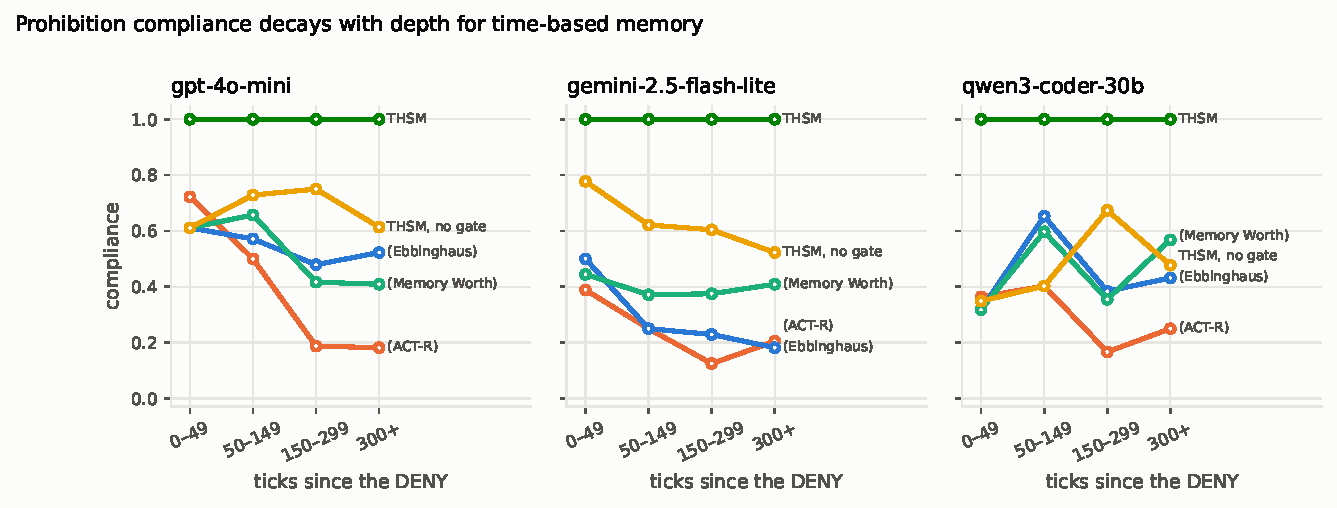
\includegraphics[width=\linewidth]{figures/fig4_depth}
\caption{Figure 4. Prohibition compliance by depth since the DENY, three models.}
\label{fig:fig4}
\end{figure}

ACT-R memory produces a clean depth curve on gpt-4o-mini, Gemini and Sonnet 5 (0.72 $\rightarrow$ 0.18, 0.39 $\rightarrow$ 0.12, 1.00 $\rightarrow$ 0.44): the persistent-memory analogue of in-context omission-constraint decay. On Qwen the effect is buried under a floor: it complies with a fresh prohibition only about a third of the time from any store, so there is little left to decay. Ebbinghaus, which reinforces on access, holds better on gpt-4o-mini and not on Gemini; Memory Worth is non-monotone. Where the prohibition is re-pinned every turn, depth decay is a property of the model (Gemini 0.78 $\rightarrow$ 0.52, gpt-4o-mini flat). The gate removes the depth dependence entirely.

\subsection{Compaction is not the main erosion path once memory persists}

\begin{table}[t]
\centering
\small
\caption{Violation rate on unauthorized probes immediately before and after a session compaction (46 bracket pairs per store, gpt-4o-mini).}
\label{tab:6}
\begin{adjustbox}{max width=\linewidth}
\begin{tabular}{lrrr}
\toprule
store & compaction & before & after \\
\midrule
type-blind & plain summary & 0.43 & 0.46 \\
type-blind & summary with permission lines pinned & 0.43 & 0.22 \\
THSM, no gate & plain summary & 0.30 & 0.22 \\
THSM, no gate & pinned & 0.30 & 0.13 \\
THSM & either & 0.00 & 0.00 \\
\bottomrule
\end{tabular}
\end{adjustbox}
\end{table}

Governance Decay reports 0\% $\rightarrow$ 30\% violations when compaction drops an in-context policy. In a memory-augmented harness the constraint is never only in the session context, and the agent was already violating it 43\% of the time before compaction; compaction moves the rate by three points. Constraint Pinning at compaction still halves post-compaction violations (0.43 $\rightarrow$ 0.22) and lowers overall false authority (0.39 $\rightarrow$ 0.29), as a recency effect: a constraint that has just been restated is followed more often. It is a mitigation, not a fix; the gate is zero under both compaction modes.

\subsection{Writer and pinning controls}

\emph{Writer.} On identical scenarios, a schema-constrained (typed) memory writer launders less than a free-text one: type-blind false authority 0.59 $\rightarrow$ 0.54, pinned-ungated 0.32 $\rightarrow$ 0.25 with revocation survival 0.61 $\rightarrow$ 0.94, and better knowledge recall (KUA 0.38 $\rightarrow$ 0.65). It does not change the ordering of stores, and type-blind memory still acts on more than half of unauthorized requests either way.

\emph{Pinning leak.} Pinned grant scopes such as \texttt{run\_cmd cmd="*test*"} leak enough of a task command that THSM can keep skill success after the skill note has decayed. With tool-name- only pinning, THSM's utility falls by 0.02--0.04 on gpt-4o-mini and by 0.07 at full decay on Gemini, with authority unchanged at zero. We therefore report THSM's utility as "within $\pm$0.05 of type-blind" rather than as a lead. Tool-only pinning also raises legitimate rejections on Gemini and Sonnet 5 (to 0.33--0.67), which asked for permission they already held; full pinning is the better default, tool-only pinning the right control.

\subsection{External validation on a skill-retention benchmark}

Continual-ARC (Hodel-style Re-ARC generators over a lifetime of recurring, drifting tasks) has no authority concept, so it cannot test the creep claims; it can test what the exemption costs. We wrote a memory-augmented learner for its own runner that stores one PROC rule per task, applies our decay policies, and re-derives an evicted rule at demo cost. Model gpt-5-mini, smoke config, 8 runs, 1024 instances.

\begin{table}[t]
\centering
\footnotesize
\caption{Continual-ARC, score and retention. "repeat" is the solve rate on non-first exposures; first-exposure solve rate is 0.25--0.50 throughout.}
\label{tab:7}
\begin{adjustbox}{max width=\linewidth}
\begin{tabular}{lrrrrrr}
\toprule
schedule & policy & score & repeat & evictions & re-derivations & rule hits \\
\midrule
isolated & none / Ebbinghaus / ACT-R (a=0.5) & 72.9 / 73.2 / 72.3 & 0.63 / 0.65 / 0.64 & 0 / 0 / 0 & 160 / 159 / 160 & 85 / 89 / 91 \\
workstreams & none & 71.1 & 0.60 & 0 & 179 & 72 \\
workstreams & Ebbinghaus a=0.5 & 71.5 & 0.59 & 1 & 174 & 73 \\
workstreams & ACT-R a=0.5 & 68.3 & 0.54 & 2 & 192 & 73 \\
workstreams & ACT-R a=0.9 & 58.3 & 0.39 & 37 & 290 & 20 \\
workstreams & ACT-R a=1.0 & 59.5 & 0.42 & 40 & 287 & 21 \\
\bottomrule
\end{tabular}
\end{adjustbox}
\end{table}

Three things follow. First, memory carries the score: repeat exposures solve at 0.59--0.65 against 0.25 on first exposure, so the benchmark measures the quantity our SSR proxies, with binary ground truth. Second, the isolated schedule is a null (all three policies within 0.9 score points, zero evictions): decay is free when recurrence is immediate. Third, in the workstreams schedule evictions, re-derivations and score move together, and the cost of forgetting is large when forgetting actually happens: 37--40 evictions drop the score by 12 points, cut rule reuse by 72\% and raise re-derivations by 60\%.

The policy asymmetry is the part that speaks to \S6.2. Ebbinghaus evicted once in 128 instances at a=0.5, and replaying the observed access sequences offline through the policy gives zero evictions even at a=1.0: its strength term is multiplicative in access count, so two or three reuses push the effective time constant past any horizon the schedule offers. Memory Worth is nearly as inert here because these rules mostly succeed. ACT-R's power-law activation is the only policy that forgets under realistic recurrence gaps --- and it is the same policy whose false authority rises monotonically with decay aggressiveness in Table 2. Creep-under-decay and retention-loss-under-decay are one mechanism observed twice: what power-law activation prunes is whatever has not been retrieved recently, which is a revocation in one benchmark and a skill in the other.

\subsection{Authority created versus authority acted on}

Every model writes deontic-looking memory: 5--65 claims per run with the typed writer (Sonnet 5 fewest, Qwen most, tracking their type-blind false authority of 0.27 and 0.58). On THSM those writes become flagged claims with no effect on A(t); on \texttt{typed\_nolabels} the same writes become 16--50 real widenings per run. Creation is a property of the model; laundering is a property of the store. Because the widened scopes were rarely probed, behavioural false authority under-reports this by construction, which is why \texttt{INV} belongs next to \texttt{FAR}.
